\documentclass{beamer}

% german content
\usepackage[ngerman]{babel}

%for Lisas PC
\usepackage[T1]{fontenc}
\usepackage[latin1]{inputenc}

% bibliography
\usepackage[
backend=biber,
style=authoryear,
citestyle=authoryear,
autocite=footnote
]{biblatex}
\addbibresource{bibliography.bib}

% images
\usepackage{graphicx}
\graphicspath{ {./images/} }

\title{Import/Export von saisonalen Produkten}
% \subtitle{}
\author[Dao, Gabele, Neidel, Neuthor, Spannbauer, Wiegandt]{
  Dao, Duc Trung \and\\
  Gabele, Jörg \and\\
  Neidel, Jonathan \and\\
  Neuthor, Marco \and\\
  Spannbauer, Daniel \and\\
  Wiegandt, Lisa-Marlen
}
\date{Januar 2021}
\institute{HTW Berlin, Angewandte Informatik}
\logo{
\includegraphics[width=1cm]{logo}}

% theme + color theme
\usetheme{Szeged}
\usecolortheme{whale}
% see: https://deic-web.uab.cat/~iblanes/beamer_gallery/index.html

\begin{document}
\frame{\titlepage}

\begin{frame}
\frametitle{Exposé}
	@Lisa
	Der Import und Export (zur Vereinfachung im Folgenden als Außenhandel benannt) von saisonellen Produkten schwankt je nach Saison des Produktes.

\end{frame}

% show all section names
\begin{frame}
\frametitle{Inhalt}
\tableofcontents
\end{frame}
% how to exclude a section from toc: https://tex.stackexchange.com/a/66633


\section{Organisation}

\begin{frame}
	\begin{center}
	{\Huge Organisation}
	\end{center}
\end{frame}

\begin{frame}
\frametitle{Soll}
exploratives Vorgehen

  \begin{itemize}
    \item grobes Thema
    \item keine Frage
  \end{itemize}
\end{frame}

\begin{frame}
\frametitle{Soll}
Aufteilung in Phasen mit klaren Deadlines

  \begin{itemize}
    \item Meetings alle 2 Wochen
  \end{itemize}

\end{frame}

\begin{frame}
\frametitle{Soll}
Aufgabenverteilung
  \begin{itemize}
    \item 2-4 Personen
    \item (abgegrenzte) Aufgabenbereiche
  \end{itemize}
\end{frame}

\begin{frame}
\frametitle{Soll}
Projektmanager
  \begin{itemize}
    \item Koordinierungsfunktion
  \end{itemize}

\end{frame}

\begin{frame}
\frametitle{Ist}
exploratives Vorgehen

  \begin{itemize}
    \item Unklarheit über:
      \begin{itemize}
        \item Ziele
        \item Vorgehen
      \end{itemize}
  \end{itemize}

\end{frame}

\begin{frame}
\frametitle{Ist}
Meetings dienten dem Zusammenführen
  \begin{itemize}
    \item kein Termingerechter Abschluss möglich
    \item Zeit teils unproduktiv
      \begin{itemize}
        \item Unklarheit
        \item zu lange Zyklen
        \item zu wenig Kommunikation
      \end{itemize}

  \end{itemize}

\end{frame}

\begin{frame}
\frametitle{Ist}
Aufgabenverteilung
  \begin{itemize}
    \item es machen nicht alle alles
      \begin{itemize}
        \item Entlastung
      \end{itemize}
    \item ungleiche Lastenverteilung
      \begin{itemize}
        \item Aufgabenbereiche ungleich intensiv
      \end{itemize}
    \item  wenn innerhalb des Aufgabenbereiches ausgegrenzt
      \begin{itemize}
        \item  mehr raus als sonst
      \end{itemize}

  \end{itemize}

\end{frame}

\begin{frame}
\frametitle{Ist}
Projektmanager
  \begin{itemize}
    \item generell positiver Einfluss
      \begin{itemize}
        \item  Redeführer
        \item  Klarheit/Struktur
        \item  Mitglieder fordern
      \end{itemize}
  \end{itemize}
\end{frame}

\begin{frame}
	\frametitle{Rollenverteilung}
	\begin{description}
		\item[Duc Trung Dao, 575477]Main Data Seeker and Preprocessor
		\item[Jörg Gabele, 571127]Master of Theorie
		\item[Jonathan Neidel, 573619]Projekt Manager
		\item[Marco Neuthor, 573738]Principal Visualizer
		\item[Daniel Spannbauer, 572836]Head of Data Processing
		\item[Lisa-Marlen Wiegandt, 572770]Editor of Chief
	\end{description}
    \end{frame}

\section{Definitionen für diese Arbeit}
\begin{frame}
	\begin{center}
		{\Huge Definitionen}
	\end{center}
\end{frame}

\begin{frame}
\frametitle{Export und Import}
	@Jörg @Trung
\end{frame}

\section{Datenbeschaffung und -aufbereitung}
\begin{frame}
	\begin{center}
		{\Huge Datenbeschaffung}
	\end{center}
\end{frame}

\begin{frame}
	\frametitle{Beginn der Datensuche}
		\begin{itemize}
			\item statistische Jahrbuch des Bundesministeriums für Ernährung und Landwirtschaft (BMEL)
			\begin{itemize}
				\item bestehend aus einzelnen Monatsberichten des jeweiligen Jahres
				\item beinhaltet themenrelevante Tabellen, wie zB Import-/Export der Kartoffelverarbeitung
				\item nur in PDF Format vorliegend
			\end{itemize}
		\end{itemize}	
\end{frame}

\begin{frame}
	\frametitle{Beginn der Datensuche}
	\begin{figure}[h]
	\caption{Beispieltabelle aus dem statistischen Jahrbuch}
	\centering
	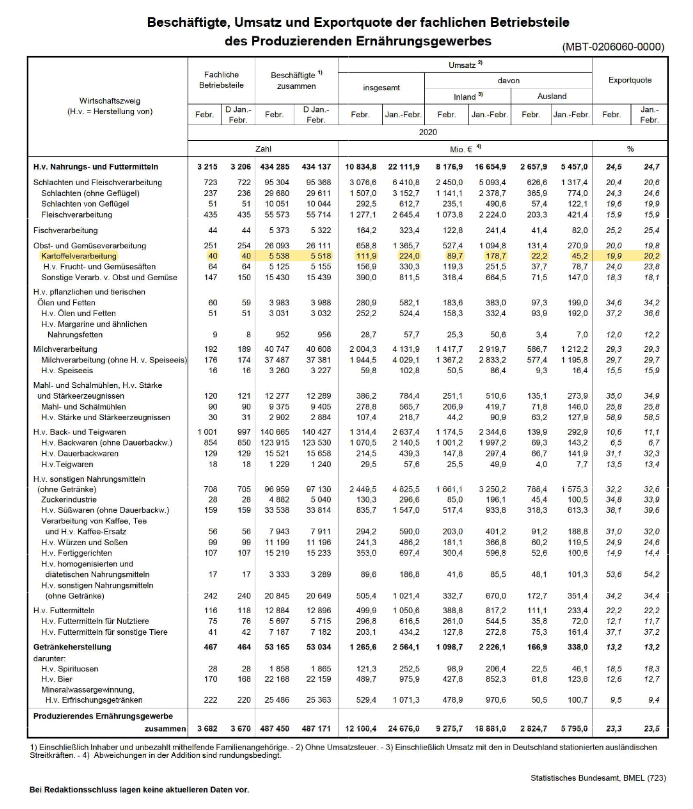
\includegraphics[scale=0.5]{3_Beispieltabelle}
		%Größe mit Daniel noch besprechen und Quellen einfügen
	\end{figure}
\end{frame}

\begin{frame}
	\frametitle{Probleme}
	\begin{itemize}
		\item Dateiformat
			\begin{itemize}
				\item Informationen per Hand exportiert
			\end{itemize}
		\item unvollständiger Datensatz
			\begin{itemize}
				\item Berichte nicht immer mit den selben Tabellen ausgestattet
				\item nicht alle Monate im Jahrbuch vorliegend
			\end{itemize}
	\end{itemize}
\end{frame}

\begin{frame}
	\frametitle{Probleme}
	\begin{figure}[h]
		\caption{unvollständige Auflistung}
		\centering
		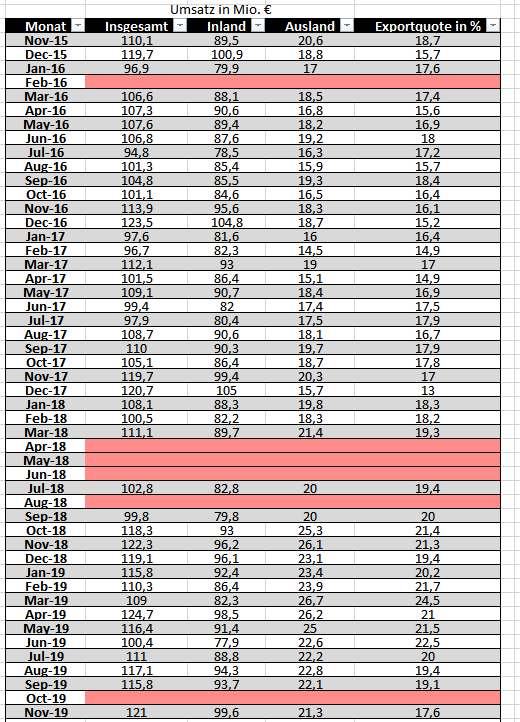
\includegraphics[scale=0.3]{4_Monatsberichte_unvoll}
	\end{figure}
\end{frame}

\begin{frame}
	\frametitle{Weitere Suche}
	\begin{itemize}
		\item statista.com
			\begin{itemize}
				\item simple Statistiken
				\item einzelne Diagramme
			\end{itemize}
	\end{itemize}
\end{frame}

\begin{frame}
	\frametitle{statista.com}
	\begin{figure}[h]
		\caption{Beispieltabelle aus statista.com}
		\centering
		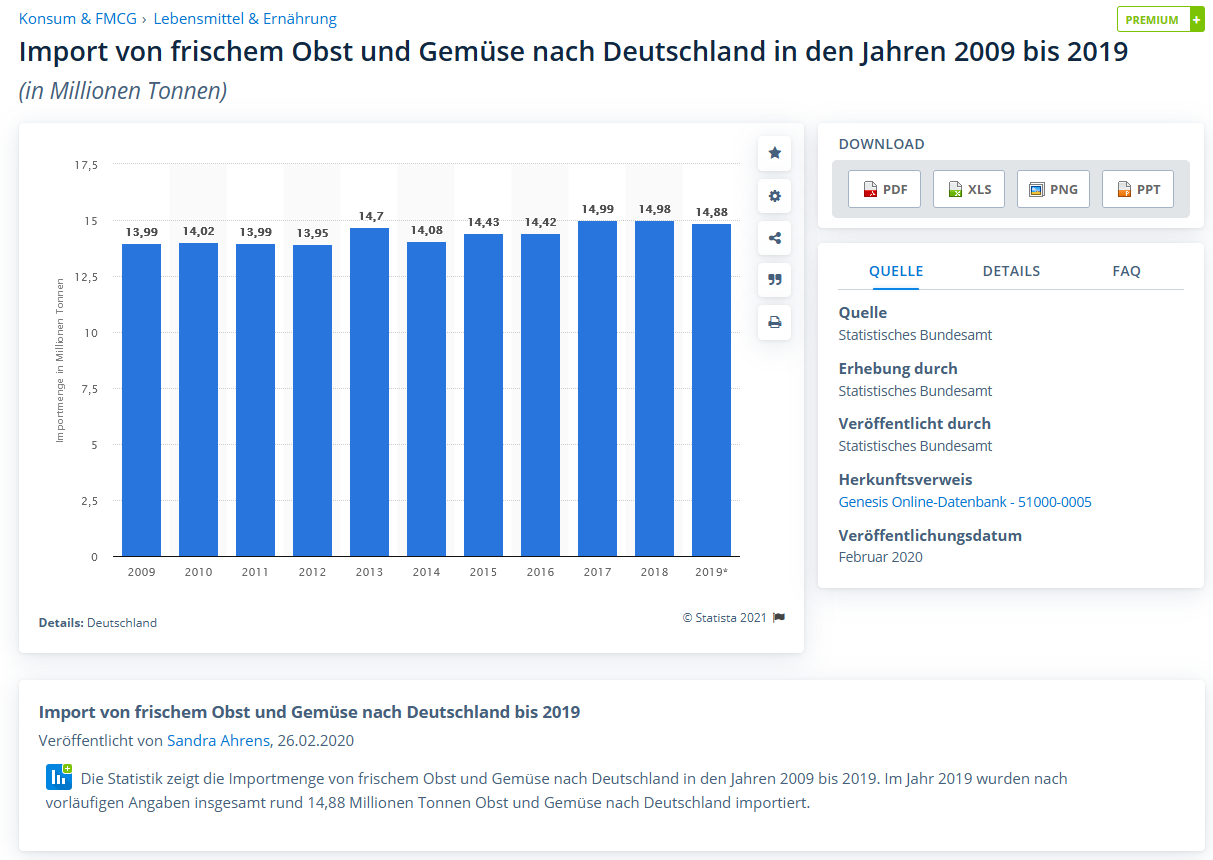
\includegraphics[scale=0.3]{5_Destatis_Report}
	\end{figure}
\end{frame}

\begin{frame}
	\frametitle{statista.com}
	\begin{figure}[h]
		\caption{Beispieltabelle von statista.com}
		\centering
		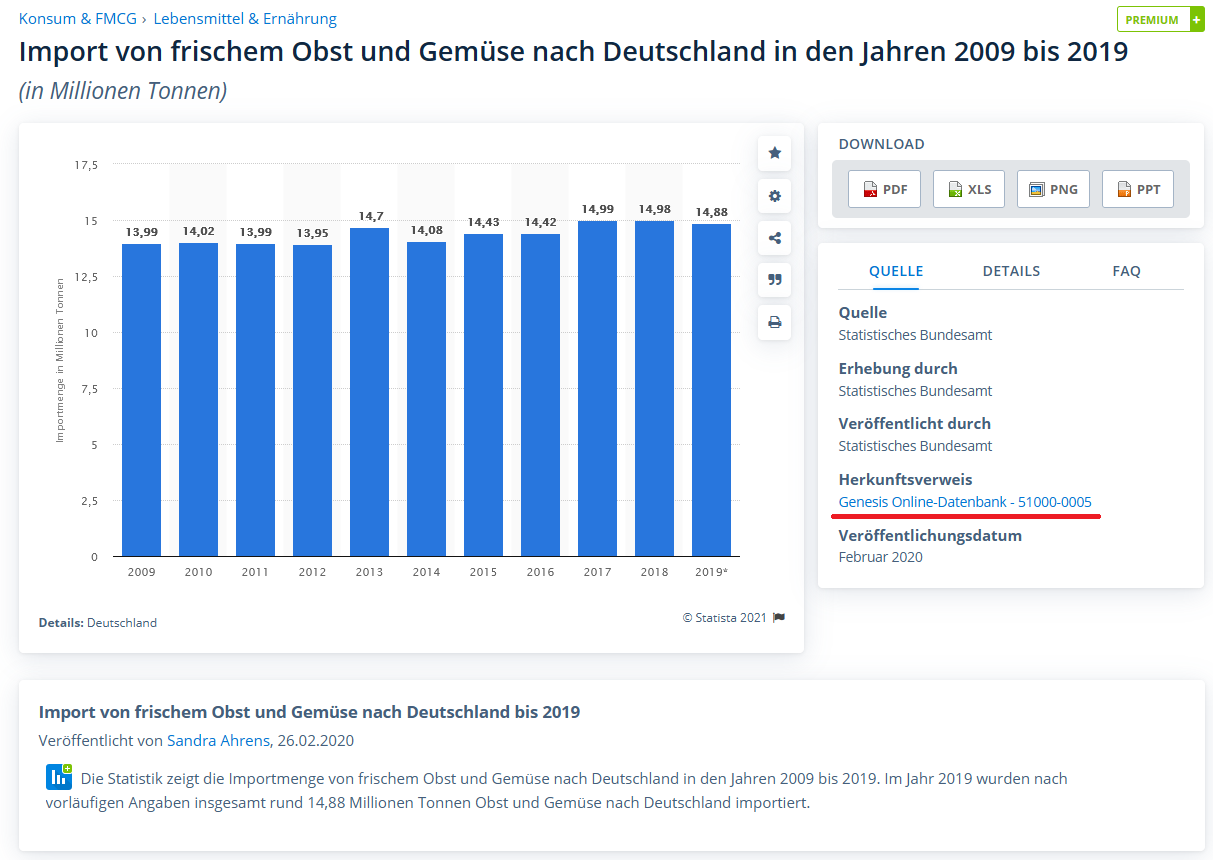
\includegraphics[scale=0.25]{5_Destatis_Report_highlightet}
	\end{figure}
\end{frame}  

\begin{frame}
	\frametitle{Lösungen}
	\begin{itemize}
		\item Analyse der Quellen
			\begin{itemize}
				\item Datenbank vom Statistischen Bundesamt (DeStatis)
			\end{itemize}
	\end{itemize}
\end{frame}

\begin{frame}
	\frametitle{Lösungen}
	\begin{figure}[h]
		\caption{Auszug der Genesis-Website}
		\centering
		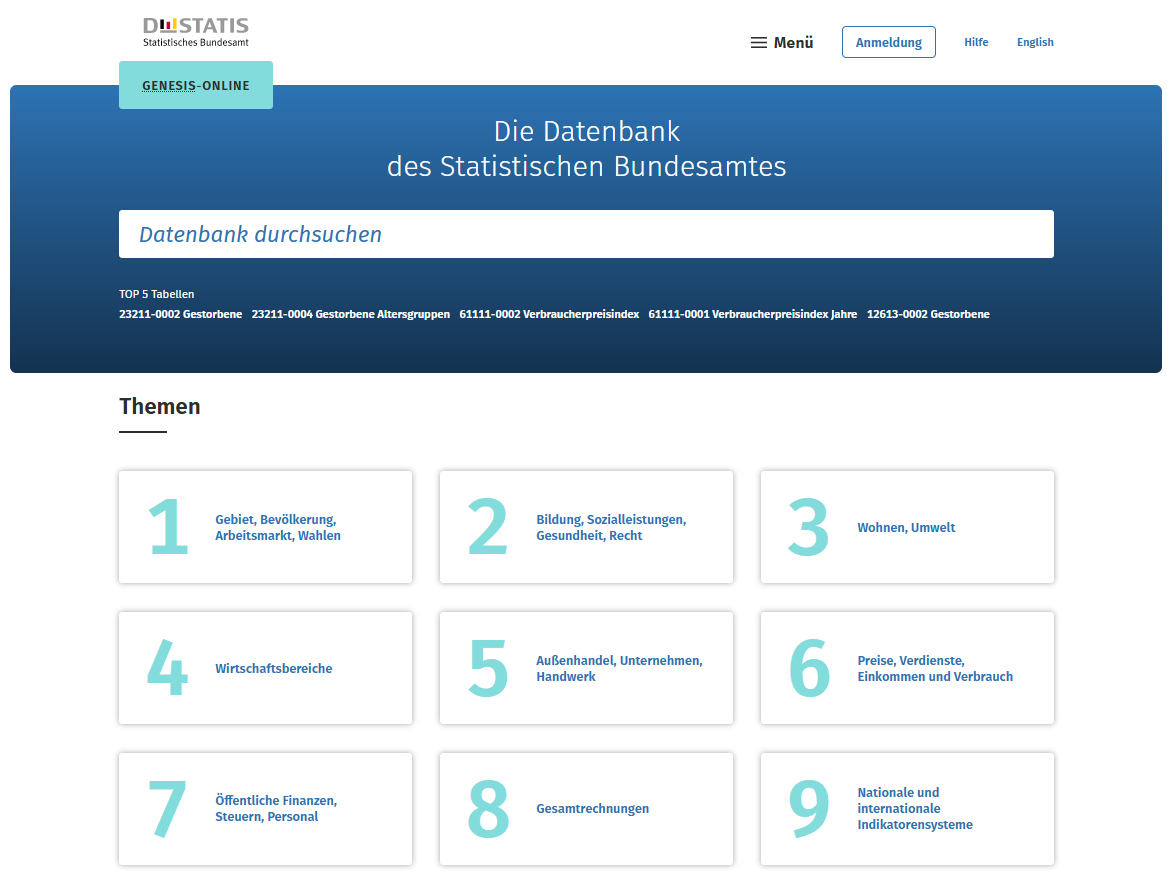
\includegraphics[scale=0.15]{6_Denesis_Destatis}
	\end{figure}
\end{frame}

\begin{frame}
	\frametitle{Lösung}
	\begin{figure}[h]
		\caption{Auszug der Tabellenübersicht von Genesis}
		\centering
		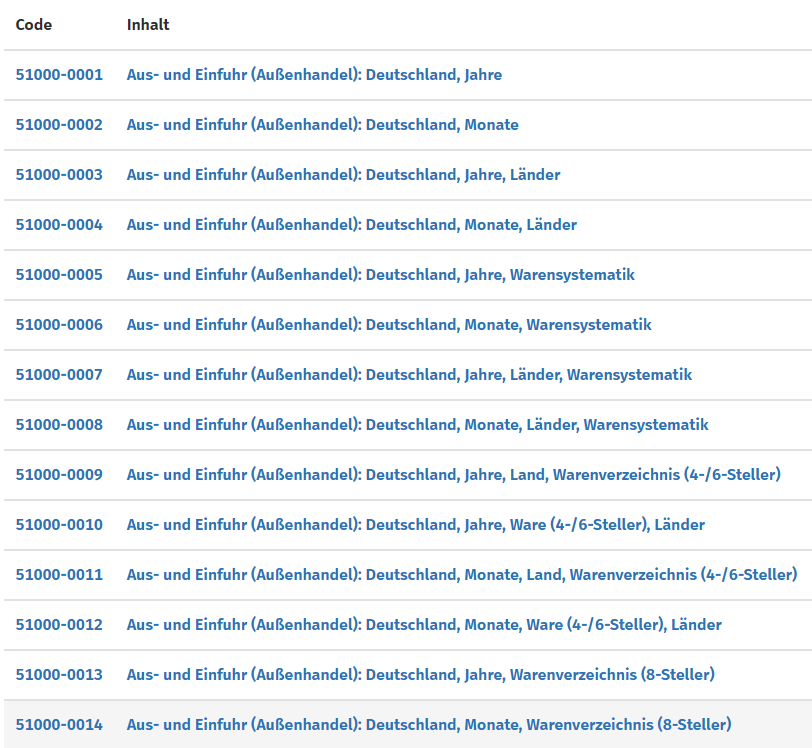
\includegraphics[scale=0.2]{8_Tabellen_codes}
	\end{figure}
\end{frame}

\begin{frame}
	\frametitle{Lösung}
	\begin{itemize}
		\item Generierung einer CSV Datei über Auswahl von relevanten Spalten/Zeilen
	\end{itemize}
\end{frame}

\begin{frame}
	\frametitle{}
	\begin{figure}[h]
		\caption{CSV Generierung auf der Genesis Website}
		\centering
		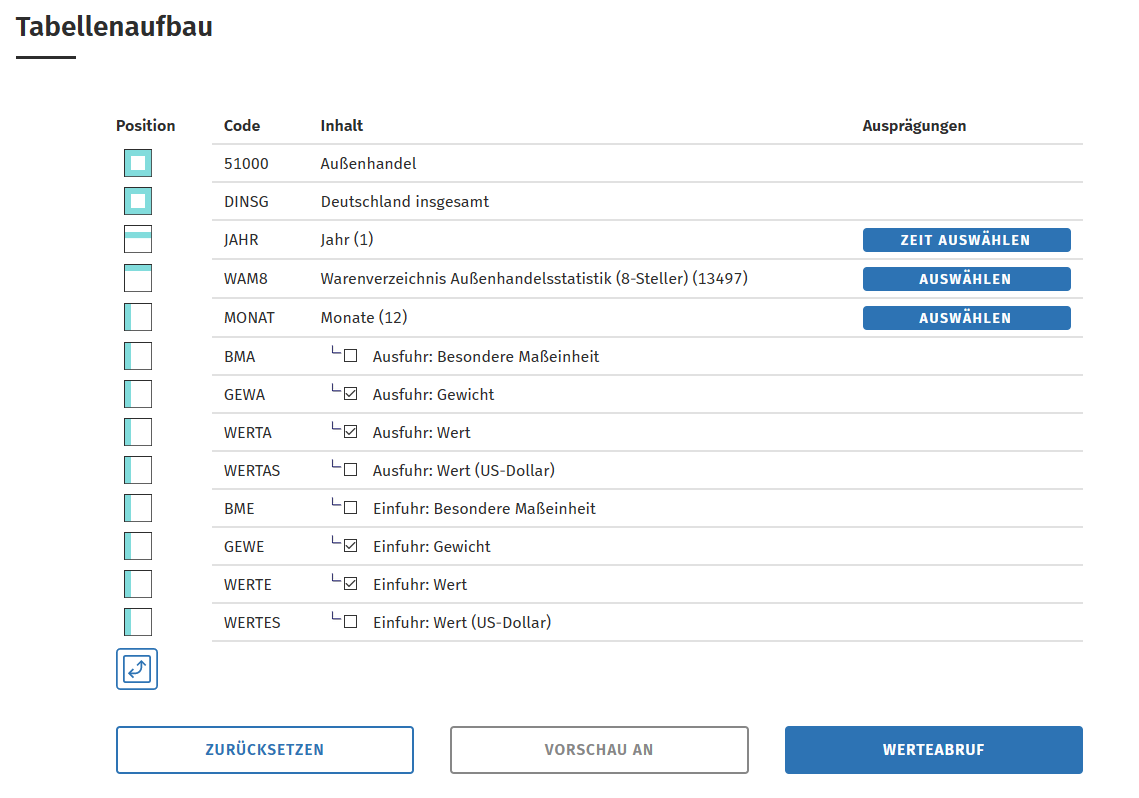
\includegraphics[scale=0.25]{9_Tabellanaufbau}
	\end{figure}
\end{frame}

\begin{frame}
	\frametitle{Lösung}
	\begin{itemize}
		\item Import in Excel
		\item anschließend grobe Aufbereitungsschritte in kleinere CSV-Dateien
	\end{itemize}
\end{frame}

\begin{frame}
	\begin{center}
		{\Huge Datenaufbereitung}
	\end{center}
\end{frame}

\begin{frame}
	\frametitle{erste Aufbereitung}
	grobe Aufbereitung der csv in Excel (Hinweis: zB leere Zeilen entfernt)
	%Screenshots?
	%achtung: nicht großer Datensatz sagen
\end{frame}
\begin{frame}
	\frametitle{Arbeit mit R}
	Arbeit mit R
	Skripte geschrieben, die Datensatz aus der csv nutzen
	%Screenshots der
\end{frame}

\section{Visualiserung}
\begin{frame}
	\begin{center}
		{\Huge Visualisierung}
	\end{center}
\end{frame}

\begin{frame}
	\frametitle{Arbeit mit R}
	@Lisa in collab w/Marco
\end{frame}

\begin{frame}
	\frametitle{Auswahl der Visualisierungsart}
	@Lisa in collab w/ Marco.
\end{frame}

\section{Informationsgewinnung}
\begin{frame}
	\begin{center}
		{\Huge Informationsgewinnung}
	\end{center}
\end{frame}

\begin{frame}
	\frametitle{Aussagen der Diagramme}
\end{frame}

\begin{frame}
	\frametitle{Aussagen der Ausarbeitung}
\end{frame}

\section{Fazit}
\begin{frame}
	\frametitle{Fazit}
\end{frame}

% bibliography
% \break
% \printbibliography

\end{document}
